\documentclass[12pt]{article}
\usepackage{rocca-homework}
\usepackage{graphicx}

\title{CS 215 Homework 5}
\author{Lucas Vas}

\begin{document}

\maketitle

\section*{Problem 1}

Shift-Store Register circuit:
\begin{center}
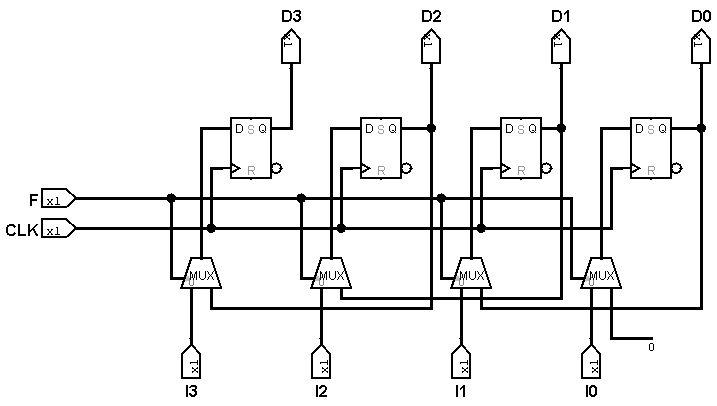
\includegraphics[width=6in]{ShiftStoreReg}
\end{center}

\clearpage

\section*{Problem 2}

Gray Code to Binary Converter circuit:
\begin{center}
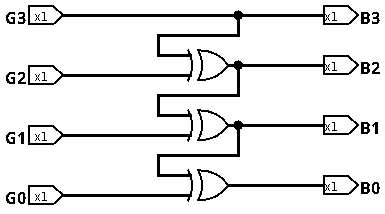
\includegraphics[width=3in]{GC2BIN}
\end{center}

Truth Table from testing:
\begin{center}
    \begin{tabular}{| c | c c |}
        \hline
        \textbf{Number} & \textbf{Gray Code} & \textbf{Binary Output} \\
        \hline\hline
        0 & 0000 & 0000 \\
        1 & 0001 & 0001 \\
        2 & 0011 & 0010 \\
        3 & 0010 & 0011 \\
        4 & 0110 & 0100 \\
        5 & 0111 & 0101 \\
        6 & 0101 & 0110 \\
        7 & 0100 & 0111 \\
        8 & 1100 & 1000 \\
        9 & 1101 & 1001 \\
        10 & 1111 & 1010 \\
        11 & 1110 & 1011 \\
        12 & 1010 & 1100 \\
        13 & 1011 & 1101 \\
        14 & 1001 & 1110 \\
        15 & 1000 & 1111 \\
        \hline
    \end{tabular}
\end{center}


\end{document}
